\chapter{Entropy Coding}
Entropy coding is a lossless data compression scheme based on symbols probability. This field was first described by Claude E. Shannon in 1948 in his paper \textit{A Mathematical Theory of Communication} \parencite{Shannon1948}.

Giving an extensive theoretical explanation of Entropy coding would require an entire thesis. Therefore, in this chapter we will define the most basic equations in Information Theory and we will also describe some well-known coding algorithms that will be relevant later. The interested reader should see reference \parencite{cover}.

\begin{figure}[h!]
	\begin{center}
		\begin{tabular}{ @{} c @{} }
			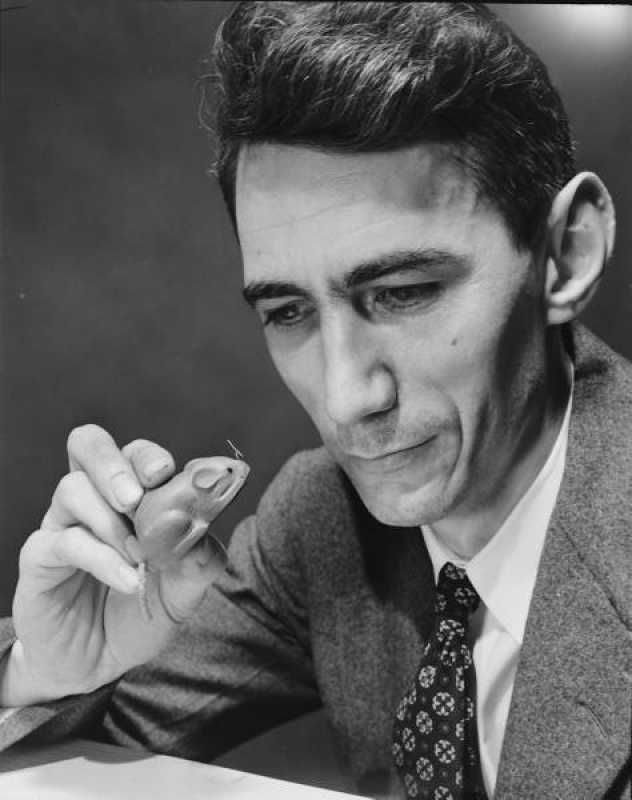
\includegraphics[scale=0.3]{images/Claude_Shannon_1776.jpg}\\
			\imagesource{DobriZheglov, CC BY-SA 4.0, via Wikimedia Commons.}
		\end{tabular}
	\end{center}
	\vspace*{-0.7em}
	\caption{Picture of Claude E. Shannon staring at a mouse.}
	\label{fig:shannon}
\end{figure}

\section{Information theory basics}
\large\textbf{Shannon entropy}

Given a discrete random variable $X$ with probability function $p(x)$, its Shannon entropy is defined as:

\begin{equation}
H(X) = - \sum_{i=1}^{n} p(x_i) \cdot \log_2 p(x_i) 
\end{equation}

This result represents the average level of information (or uncertainty) of the random variable $X$. It is expressed in \textit{bits}.\\


\large\textbf{Shannon's source coding theorem}

Shannon's source coding theorem establishes the theoretical limits to data compression, and a different meaning to Shannon entropy defined above. Formally, it states:

\begin{theorem}
Let $L_n^*$ be the expected codeword length per symbol of an optimal n-th order lossless data compression code (in bits/symbol). Then

\begin{equation}
	H(X) \leq L_n^* < H(X) + \frac{1}{n}
\end{equation}

If we took the limit when $n \to \infty$:
\begin{equation}
	\lim_{n \to \infty} L_n^* = H(X)
\end{equation}

Notice that the previous limit only exists if the source is stationary.
\end{theorem}

This theorem reveals a new interpretation of Shannon entropy: it is the average number of bits per symbol required to encode it.

\section{Huffman coding}
\begin{comment}
Òptim, prefix, FLAC, etc. Es compararà amb l'algoritme WAVE de FAPEC a través del rendiment de FLAC per àudio lossless.
\end{comment}

\section{Golomb coding}
\begin{comment}
Els codis de Rice (subconjunt dels codis de Golomb) van donar origen a FAPEC, així que és important comentar-los.
També són codis de prefix com el Huffman però poden no ser òptims.
\end{comment}

\section{Arithmetic coding}
\begin{comment}
Aquesta secció la faré servir per donar pas a l'Asymmetric numeral systems. Bàsicament els codis aritmètics són molt bons però són molt lents. Això ho compensa els ANS.
\end{comment}

\section{Asymmetric Numeral Systems}
\begin{comment}
Em centraré especialment en el Zstandard (Facebook). Tenen nivells de compressió similars als aritmètics però van MOLT ràpid (una mica més que FAPEC i tot).
\end{comment}